\chapter{Architecture Evaluation}
\label{chap:arch-eval}
This chapter focuses on architecture evaluation. The chapter will define how an alternative architecture generated by SA and GRASP is evaluated. The objective function consists of three parts: graph connectivity, scheduling of the application onto the architecture and the cost of the architecture. These three parts will be explained in detail in this chapter.

\section{Objective Function}
Before evaluating an architecture the set of fault scenarios, $\mathcal{FS}$, must be randomly generated from the fault model $\mathcal{Z} = (\mathcal{VF}, \mathcal{CF}, v, c)$. The number of fault scenarios is given by the designer. The generated fault scenarios are iterated and each iteration applies a fault scenario to the architecture, i.e. the faults in the fault scenario are injected into the architecture (see \autoref{fig:faultscenario}). In each iteration the connectivity of the architecture, $ft$, and the finish time, $\delta$, of the application on the architecture are determined. The architecture evaluation is then the sum of three variables.
$$Objective(\mathcal{A}) = \left(\displaystyle\sum_{f \in \mathcal{FS}}^{\mathcal{FS}}{\neg ft}\right) \times W_{ft} + \left(\displaystyle\sum_{f \in \mathcal{FS}}^{\mathcal{FS}}{max(0, \delta - d_{\mathcal{G}})}\right) \times W_{s} + Cost_{\mathcal{A}}$$

$\left(\displaystyle\sum_{f \in \mathcal{FS}}^{\mathcal{FS}}{\neg ft}\right)$ is the number of fault scenarios that causes the architecture to not be connected. Connectivity is denoted by $ft$ where $ft$ will be 1 if the architecture is connected and 0 if it is not connected. The number is then multiplied with $W_{ft}$ which denotes a penalty value for the connectivity. Consequently this variable will become smaller the more fault scenarios that pass the connectivity test. The penalty value $W_{ft}$ is specified as 10000.

$\left(\displaystyle\sum_{f \in \mathcal{FS}}^{\mathcal{FS}}{max(0, \delta - d_{\mathcal{G}})}\right)$ denotes the scheduling of the application on the architecture affected by the different fault scenarios. In each fault scenario the maximum of either 0 or the application finish time minus the application deadline is added to the sum. Thereby the sum grows larger as the application is not schedulable on the architecture or if it completes after the deadline. The sum is then multiplied with $W_s$ which denotes a penalty value for the schedule. Therefore the variable will grow larger as the application is not able to complete within its deadline or no schedule has been found. The penalty value $W_s$ is defined as 5000.

$Cost_{\mathcal{A}}$ denotes the physical constraints. This variable is the sum of the total number of valves and the total number of channels in the architecture.

\begin{figure}
\centering
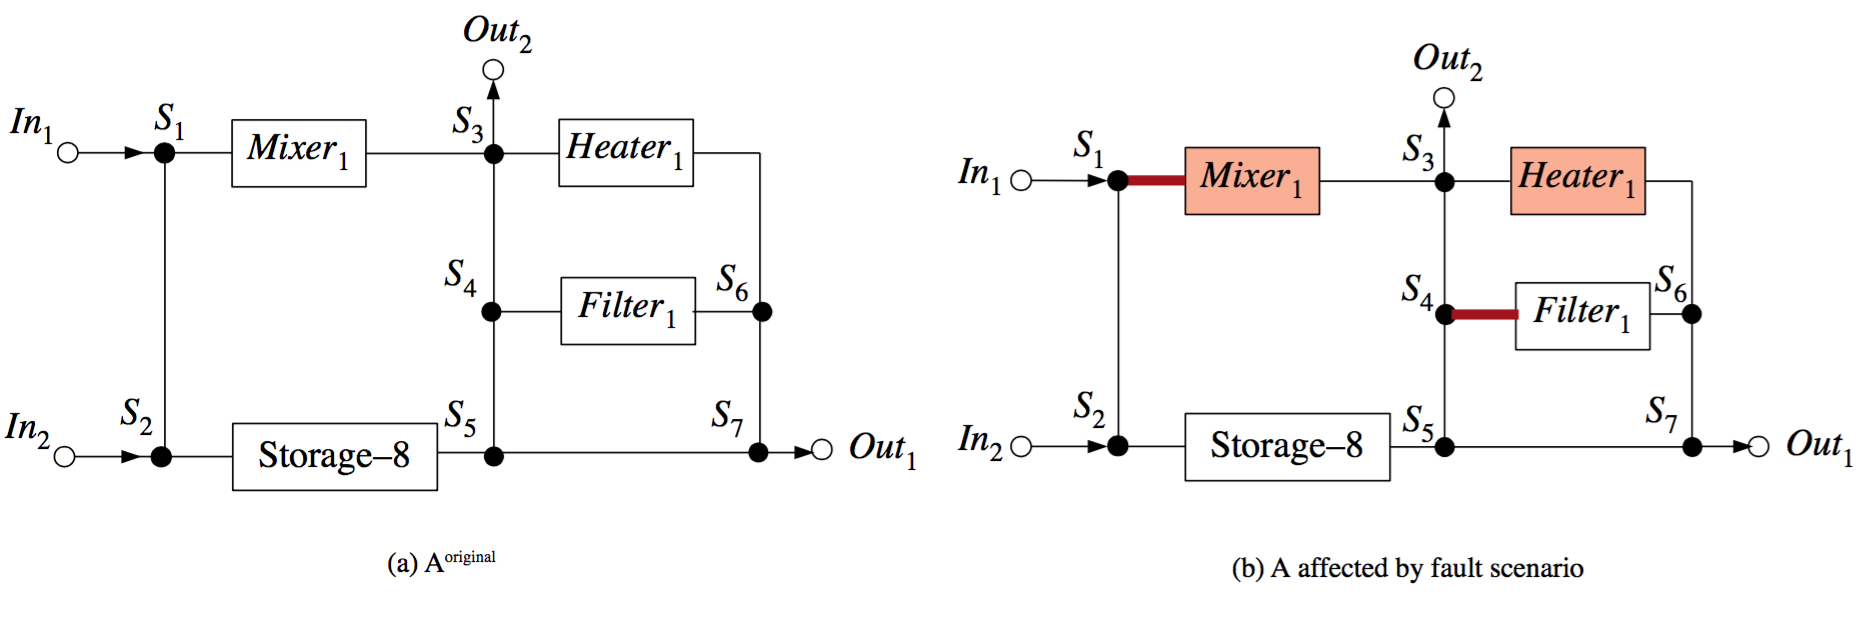
\includegraphics[width=\textwidth]{figures/faultscenario.png}
\caption[Architecture affected by fault scenario]{Architecture affected by fault scenario}
\label{fig:faultscenario}
\end{figure}

Let us consider \autoref{fig:faultscenario}a as the architecture to be evaluated, $\mathcal{A}^{original}$. Consider the fault scenario, where the channel $S_1 \rightarrow Mixer_1$ is blocked and the channel of $Heater_1$ suffers from a block defect. Additionally valves $v_6$ (a valve in the pump) of $Mixer_1$, $v_1$ (channel towards $S_3$) and $v_3$ (channel towards $S_5$) of $S_4$ are stuck open. The effects of this fault scenario is shown in \autoref{fig:faultscenario}b, where channels marked with a thick red line represent unusable channels and components marked with red are unable to perform their operation. Therefore we are unable to perform mixing, heating and route to $Filter_1$. This injection of the faults in a fault scenario is done for all generated fault scenarios, and the connectivity and scheduling are determined for each fault scenario.

The following sections will describe how the fault scenarios are generated, how the connectivity of the architecture is determined and how scheduling the application onto the architecture is done.

\section{Generation of Fault Scenarios}
\label{sec:fs-gen}
The fault scenarios, $\mathcal{FS}$, are randomly generated from the fault model $\mathcal{Z} = (\mathcal{VF}, \mathcal{CF}, v, c)$. A fault scenario $f \in \mathcal{FS}$ is a set of faults containing a set of valve faults from the set of valve faults, $\mathcal{VF}$, in the fault model and a set of channel faults from the set of channel faults, $\mathcal{CF}$, in the fault model. The fault scenarios are generated such that they are unique, i.e. $f \in \mathcal{FS}$ will occur once and only once.

The random generation of fault scenarios is divided into two phases.\\
\begin{description}
\item[First phase] The first phase consists of generating all the possible combinations of subsets of both the set of valve faults, $\mathcal{VF}$, and the set of channel faults, $\mathcal{CF}$. Recall that $v$ is the maximum number of valve faults happening in the architecture at any point and likewise $c$ is the maximum number of channel faults. Therefore all permutations of the set of valve faults needs to be generated where cardinality of the subsets are $0 \leq k \leq v$. Likewise for the set of channel faults where the cardinality of the subsets are $0 \leq j \leq c$.

\item[Second phase] The second phase picks a random subset from all the possible combinations of subsets of valve faults. Similarly it picks a random subset from the subsets of channel faults. Combining these two subsets constitutes a fault scenario, $f \in \mathcal{FS}$. This continues until the specified number of fault scenarios to generate are generated.

\end{description}

Normally we would have to use all the fault scenarios when doing the tests for connectivity and scheduling. However, as these are too numerous we have decided to use a subset. By virtue of this we are not guaranteed to create a fault-tolerant architecture which is fault-tolerant to all scenarios. However, our argument is that by using a subset, we can synthesise an architecture that can tolerate most of the fault scenarios. This argument has been investigated in \autoref{chap:exp-eval}. However, it is not a problem if an architecture is not fault-tolerant. As mentioned in \autoref{sec:prob-for} this tool is part of a methodology. If after testing we determine that a fault, which is not tolerated, is present, we will discard the chip.

The implementation of the generation of fault scenarios is shown in \autoref{alg:fault-gen-algo}. $NoFS$ is the number of fault scenarios to be generated.

\begin{figure}[H]
\centering
\begin{algorithmic}[1]
\Function{GenerateFaultScenarios}{$\mathcal{Z}, NoFS$}
	\State $vsubsets \gets \Call{PossibleCombinations}{\mathcal{VF}, v}$\Comment{Phase 1}
	\State $csubsets \gets \Call{PossibleCombinations}{\mathcal{CF}, c}$
	\State $i \gets 0$
	\State $\mathcal{FS} \gets \emptyset$
      \While{$i < NoFS$}\Comment{Phase 2}
        \State $v \gets \Call{RandomSet}{vsubsets}$
        \State $c \gets \Call{RandomSet}{csubsets}$
        \State $f \gets v \cup c$
	\If{$f \notin \mathcal{FS}$}\Comment{If the fault scenario does not exist add it to $\mathcal{FS}$}
		\State $\mathcal{FS}.\Call{add}{f}$
		\State $i \gets i + 1$
	\EndIf
      \EndWhile
      \State \textbf{return} $\mathcal{FS}$
    \EndFunction

\Function{PossibleCombinations}{$set, k$}
	\State $j \gets 1$
	\State $subsets \gets \emptyset$
	\While{$j \leq k$}
		\State $r \gets \Call{permutations}{set, j)}$
		\State $subsets.\Call{add}{r}$
	\EndWhile
	\State $subsets.\Call{add}{\emptyset}$\Comment{Remember that the empty set (no faults) is possible}
	\State \textbf{return} $subsets$
\EndFunction
\end{algorithmic}
\caption[Implementation of random generation of fault scenarios]{Implementation of random generation of fault scenarios}
\label{alg:fault-gen-algo}
\end{figure}

\section{Connectivity}
\begin{figure}
\centering
\begin{algorithmic}[1]
\Function{IsConnected}{$\mathcal{A}$}
	\State $start \gets \Call{ChooseRandomInput}{\mathcal{A}}$
	\State $visited \gets \emptyset$\Comment{Keep track of the visited components}
	\State $Q.\Call{enqueue}{start}$\Comment{$Q$ is a FIFO queue}
	\State $visited.\Call{add}{start}$
      \While{$Q$ is not empty}
        \State $v \gets Q.\Call{dequeue}{\null}$
	\ForAll{connection from v to w in $\mathcal{A}$.OutConnections(v)}
		\If{connection not faulty and $w \notin visited$}
		\State $visited.\Call{add}{w}$
		\State $Q.\Call{enqueue}{w}$
		\EndIf
	\EndFor
      \EndWhile
	%\State $inputs \gets \mathcal{A}.inputs$ \textbackslash ${}$ $start$\Comment{A set containing all components excluding inputs}
	\If{($\mathcal{N}$ $\backslash$ $\mathcal{A}.inputs$) $\in visited$}\Comment{If all vertices $N \in \mathcal{N}$ excluding inputs are in the $visited$ set. The architecture is connected}
		\State \textbf{return} true
	\Else
		\State \textbf{return} false
	\EndIf
    \EndFunction
\end{algorithmic}
\caption[Implementation of graph connectivity algorithm]{Implementation of graph connectivity algorithm}
\label{alg:connectivity}
\end{figure}
Due to permanent faults, an architecture can become disconnected and thereby routing of fluid to the desired destination is no longer possible. Therefore it is important that an architecture is connected. The initial architecture given by the designer is assumed to be connected. The connectivity of the architecture is determined by using the algorithm Breadth First Search or \emph{BFS} for short. BFS is an algorithm for traversing a graph data structure. The BFS algorithm starts at one of the input nodes and traverses the architecture. If BFS visits all the components, excluding the input nodes, in the architecture then the architecture is connected. The input nodes are excluded due to being a source of input and they never receive any fluid from other components on the chip. Contrary if some components are not visited by the BFS then the architecture is not connected. The implementation considers connections (channels) that are blocked and switches that are affected by a valve fault and therefore have their routing affected. The implementation of the BFS algorithm is shown in \autoref{alg:connectivity}. If in a given fault scenario a switch is suffering from more than one valve fault that causes it to disallow fluid going to a certain component the affected connection is deemed faulty and removed from the architecture while being affected by that fault scenario. It is added again to the architecture when the architecture is restored from being affected by the fault scenario. Similarly blocked channels are considered. Therefore the implementation shown in \autoref{alg:connectivity} is possible. The connectivity test is done for each fault scenario in the set of generated fault scenarios.

%The function $PossibleConnection(from_component, to_component)$ is a function that returns the connections that are possible to use coming from a component ($from_component$) to ($to_component$), i.e. if a channel is blocked it is not usable and likewise what connections are usable in a switch affected by valve fault(s).

%pseudo code

\section{List Scheduling}
\label{sec:list-scheduling}
An architecture is only fault-tolerant if it can run the application within its deadline. To determine the finishing time of the application, on a given architecture affected by a fault scenario, we use the List Scheduling Algorithm, henceforth \emph{LS}. Mapping the application onto the architecture involves binding of operations onto the allocated components, scheduling the operations and performing the required fluidic routing as outlined in \autoref{sec:app-map}. LS is a heuristic approach to solve the problem of application mapping in a computationally efficient manner. Together with the operation binding and scheduling, the heuristic approach also considers the fluidic routing and channel contention. The input to this tool is a netlist, which is not yet routed, i.e. the physical placement of components is not known yet. We only know the exact routing latencies if we know the routes. However, the routing latencies should not be completely ignored when determining a schedule using LS. Therefore we assume that the designer gives an average latency, which we use when determining a schedule. This may mean that the application is actually not schedulable as we could be using routing latencies, which are smaller than those resulted after the physical synthesis. However it is still a reasonable estimation of the application completion time. In case the application is actually not schedulable, this will be known after the testing, when we have the physical architecture. If the application turns out not to be schedulable, the chip is discarded.

\begin{figure}
\centering
\begin{algorithmic}[1]
\Function{ListScheduling}{$\mathcal{A}, \mathcal{G}$}
	\State $PQ.\Call{put}{\mathcal{G}.source}$\Comment{$PQ$ is a priority queue}
      \While{$PQ$ is not empty}
        \State $o \gets PQ.\Call{ExtractMax}{\null}$
	\State $success \gets \Call{BindAndSchedule}{o}$
	\If{$success$ is true}
		\ForAll{$op \in$ \Call{ReadySuccessors}{o}}
			\State $PQ.\Call{put}{op}$
		\EndFor
	\Else
		\State \textbf{return} $d_\mathcal{G} \times 2$ \Comment{No schedule is found and a high value is returned to make the cost of the architecture higher}
	\EndIf
      \EndWhile
	\State \textbf{return} $\mathcal{G}.sink.finishtime$
    \EndFunction

\Function{BindAndSchedule}{$operation$}
	\State $time \gets \infty$
	\State $best \gets null$
	\State $components \gets \mathcal{A}.\Call{GetComponentsForOperation}{operation}$\Comment{The architecture keeps track of faulty components}
	\ForAll{$component \in components$}
		\State $t = \Call{ReadyTime}{operation, component}$
		\If{$t < time$}
			\State $time \gets t$
			\State $best \gets component$
		\EndIf
	\If{$best \neq null$}
		\State \Call{ScheduleOperation}{$operation$, $best$}\Comment{This also schedules the edges and renders the channels unusable while the operation is using them}
		\State \textbf{return} true
	\Else
		\State \textbf{return} false\Comment{The operation is not possible to schedule}
	\EndIf
	\EndFor
\EndFunction
\end{algorithmic}
\caption[Implementation of the List Scheduling algorithm]{Implementation of the List Scheduling algorithm}
\label{alg:list-scheduling}
\end{figure}

LS is a while loop that runs until all operations ($\mathcal{O}$) and edges ($\mathcal{E}$) from the application ($\mathcal{G}$) are scheduled. The operations are topologically sorted based on the dependency constraints. At each step a ready operation and its edges are bound and scheduled to a component. The algorithm tries all possible bindings and chooses a binding that produces the shortest completion time for that operation. The list of ready operations are prioritised using the urgency criteria. The urgency of an operation is specified as the length of the longest path from the operation to the sink, i.e. summing the execution weights of the vertices. When an operation has been scheduled its ready successor operations are added to the list of ready operations. If no component is found during the binding then there is no schedule for the application on the architecture. If the number of ready operations exceeds the number of available resources the most urgent operations are scheduled and the remaining ones are deferred. Ready operations are defined as operations whose predecessors have completed. Determining routes between components is done by using BFS where the BFS considers channels affected by faults and switches affected by valve faults as when determining the connectivity.

The implementation of LS in this thesis is given in \autoref{alg:list-scheduling}. The application is preprocessed such that two operations are added with execution times of 0. Recall the application $\mathcal{G}$ has a source and a sink as shown in \autoref{fig:application}. These two operations are added where the source is added such that all the operations which originally had no dependencies (input operations) depend on the source operation. Contrary the sink is added such that all operations who originally no other operation depended on (output operations), the sink operation depends on the completion of them. Thereby the completion time of the application graph $\mathcal{G}$ onto the architecture $\mathcal{A}$ is the finish time of the sink operation. Furthermore the source operation provides the LS algorithm with a starting point.

In the $BindAndSchedule()$ function the algorithm tries all the possible bindings for an operation and chooses the one that produces the shortest completion time for the operation. It also considers the routing time and routing constraints. If the component is occupied by another operation it will consider the time it takes for the operation occupying the component to route to the storage. Therefore a storage reservoir is only used if the component to which the previous operation was bound is needed for performing another operation. The function $ScheduleOperation()$ then schedules the operation on the component specified. It also binds and schedules the edges such that the channel(s) used by the edges cannot be used by other edges during that time. The operation also schedules the flows to storage if needed for the previous operation occupying the component. If no route can be found to a component needed by the operation or if no component is able to perform that operation then no schedule exists and the LS algorithm returns the a high value to make the cost of the architecture higher, i.e. $d_\mathcal{G} \times 2$.


\section{Summary}
This chapter defines how an architecture is evaluated. The architecture is evaluated by determining if the architecture is connected and if the application is able to finish within its deadline when affected by a fault scenario in the set of generated fault scenarios. Connectivity of the architecture is determined using the algorithm Breadth First Search. The schedule for the application graph on the architecture is determined using the List Scheduling algorithm. The fault scenarios are generated at random from the fault model where the number of generated fault scenarios is determined by the designer. Additionally the objective function also considers the physical constraints of the architecture, which is the number of valves and channels (connections) in the architecture.
